% ==================================================
% CHAPTER 5: Using cosmic muons to measure relative strip position offsets %
% ==================================================

\chapter{Using cosmic muons to measure relative strip position offsets}
\label{chap:cosmics}
% Edit count: Lia - 0, Brigitte - 0

At McGill, among other quality and functionality tests, each Canadian-made quadruplet was characterized with cosmic muons. In this chapter, the experimental setup and how the data was analyzed to provide relative strip position offsets is presented. The analysis method was motivated by the how it could be compared to data collected with the x-ray method (chapter~\ref{chap:xray}) but also stands alone as a characterization of the alignment between strips of different layers. First, a brief introduction to cosmic rays.

% --------------------------------------------------
\section{Cosmic rays}
% --------------------------------------------------

The Earth is being bombarded by particles from the sun, galactic sources and extra galactic sources~-- collectively called cosmic rays~\cite{boezio_chemical_2012, zyla_review_2020}. Cosmic rays are mostly protons, but also heavier ions, gamma rays and the term sometimes includes neutrinos. The primary (initial) cosmic ray interacts with the atmosphere causes electromagnetic and hadronic showers of particles. Hadronic showers result from the primary cosmic ray interacting strongly with the target of the atmosphere and the most abundant products are pions. Charge pions mostly decay to muons (there is a lesser contribution to the muon flux from kaons as well)~\cite{grieder_cosmic_2001}. Thanks to time dilation extending the muon's lifetime as measured on Earth, a flux of approximately 1 muon\SI{}{\per\cm\squared\per\min} reaches the ground~\cite{zyla_review_2020}. Measuring the muon flux and energy spectrum reveals information about primary cosmic rays~\cite{grieder_cosmic_2001} which is interesting to high energy physicists and astrophysicists. The muon flux is also terribly convenient for testing muon detectors.

% --------------------------------------------------
\section{Experimental setup}
% --------------------------------------------------

Cosmic muon characterization was done with a hodoscope, a complete description of which can be found in~\cite{lefebvre_thesis}.  The quadruplet was placed in the center of the test bench. Above and below it was a layer of scintillator-PMT arrays, labeled in figure~\ref{fig:hodoscope}. When a cosmic muon passed within the acceptance of the hodoscope, at least one scintillator from the top array and at least one from the bottom array fired in coincidence. The coincident signal was used to trigger the readout of the quadruplet's electrodes using NIM modules. The trigger was passed \iffalse through a KC705\footnote{Xilinx, Xilinx Kintex-7 FPGA KC705 Evaluation Kit, EK-K7-KC705-G, 2018} which sent it \fi to the front-end electronics attached to the adaptor boards of each layer of the quadruplet.

\begin{figure}
    \centering
    \includegraphics[width = 0.9\textwidth]{figures/figure_test_bench.png}
    \caption{Cosmic muon hodoscope at McGill University with sTGC quadruplet in the test bench.}
    \label{fig:hodoscope}
\end{figure}

Operating the chambers also required gas and high voltage. A pentane-CO$_{2}$ mixture was mixed and delivered to each sTGC with a gas system designed and made at McGill University. The gas system was controlled by a slow control program, also made in-laboratory~\cite{keyes_development_2017}. Although gas mixture is flammable, it allows the chambers to operate in high amplification mode without prodution of excess photons saturating the signal across many strips because pentane absorbs a wide energy of photons~\cite{majewski_thin_1983}.  To prepare the quadruplets for operation, CO$_{2}$ was flushed through them overnight to remove impurities. Then, five gas volumes of the pentane-CO$_{2}$ mixture was flushed through (approximately 3 hours). High voltage was provided by CAEN boards. 

% About 2.9 kV vs 3.1 kV
%Although the chambers will be operated at 2.8~kV in ATLAS, the earlier version of the FEBs used at McGill had a worse signal-to-noise ratio for pads, which was compensated for operating the chambers at 3.1~kV, which increased the chambers' gain. Operating at 2.9~kV was sufficient for strip and wire signals and closer to the nominal voltage. Collecting 1 million triggers at each voltage provided enough statistics to calculate characterization metrics, which meant collecting data for just over two hours per quadruplet per voltage.

% --------------------------------------------------
\section{Data acquisition}
% --------------------------------------------------
% It would be great to have a scope trace here, preferably of a strip. Oops.
Each sTGC electrode was connected to a channel on a prototype ASIC\footnote{the VMM3~\cite{iakovidis_vmm3_2017}, designed for the MMs and sTGCs of the NSW} on the front-end electronics, attached to the adaptor boards on each layer of a quadruplet.  The ASIC amplified the signal and was set to measure and record the signal peak amplitude from electrodes. For each trigger, the signal peak amplitude of all channels above threshold was recorded as an event and stored in a binary file. Channel thresholds were estimated~\cite{chen_calibration_2019} and adjusted manually in the configuration/readout software before the start of data acquisition. There was an exception to the threshold rule: the signals on strips adjacent to a strip above threshold were also readout using the so-called``neighbour triggering'' function of the ASIC. 

The quadruplets were held at 3.1~kV for approximately two hours to collect data from 1 million muon triggers.

% --------------------------------------------------
\section{Data preparation}
% --------------------------------------------------
\subsection{Cuts on electrode hits}
Corrupted data is removed while the raw data is being recorded in a binary file. The binary file is decoded into a usable \package{ROOT}~\cite{ROOT_paper} tree offline. 

A hit is defined as a signal recorded from a channel that was above threshold or (in the case of strips) neighbour triggered. In addition to hits from muons, the quadruplets record noise from the electronics and $\delta$-rays (electrons liberated with sufficient energy to cause more ionization before acceleration). Therefore, cuts are applied to reduce the number of noise hits. The edge strips are very noisy, so all strip hits on layers with strip hits on either edge channel are cut. A default pedestal value is subtracted from the recorded signal peak amplitude of each electrode for a more realistic estimate of the signal amplitude. Also, events that only have hits on pad electrodes (no strips or wires) were cut because the large area of the pads made them susceptible to noise.

% --------------------------------------------------
\subsection{Clustering and tracking}
% --------------------------------------------------

Many of the high-level characterization metrics require rebuilding muon tracks. For events passing quality cuts, the $x$- and $y$-coordinates of the ionization avalanche on each layer are extracted from the signal on the wires and strips respectively for each event, as is sketched in figure~\ref{fig:mwpc_coords}. In this work, $x$ is the coordinate perpendicular to the wires and $y$ is the coordinate perpendicular to the strips.

The $x$-coordinate is taken as the center of the wire group with the maximum peak signal amplitude, since the wire groups' pitch (\SI{36}{\milli\meter}) is larger than the typical charge spreading. Assuming that the true $x$-position of the hit is sampled from a uniform distribution over the width of the wire group, the uncertainty in the x-position was given by $\frac{36}{\sqrt{12}}$~mm~=~10~mm~\cite{Sauli:117989}.

The $y$-coordinate is taken as the Gaussian mean of the peak signal amplitude distribution across groups of contiguous strips. The process of grouping contiguous strip hits on a layer is called clustering, and the resulting group is called a cluster. Figure~\ref{fig:mwpc_coords} sketches the clustering process and a sample cluster is shown in figure~\ref{fig:sample_cluster}. The data acquisition system recorded the electrode ID of the strip hit and in the clustering process the position of the center of the strip electrode is calculated based on the nominal quadruplet geometry. Typically, clusters are built of 3-5 strips. The thickness of the graphite coating over the cathode boards determined how many strips picked up the ionization image charge. Larger clusters were more likely caused by $\delta$-rays since they spread the cloud of ionization. 

\begin{figure}
    \centering
    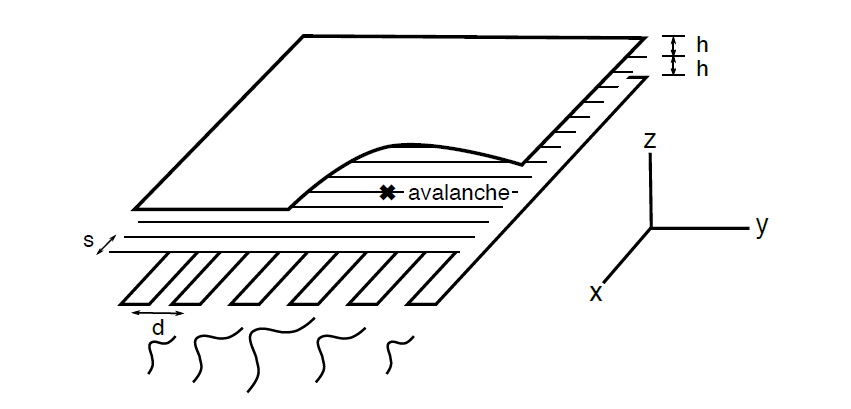
\includegraphics[width = 0.7\textwidth]{figures/mwpc_lefebvre_thesis_gatti.png}
    \caption{A sketch of an sTGC-like detector. The position of the avalanche is extracted from the wires and strips that picked up the avalanche signal. The signals on individual strips are sketched. Clustering was the processs of fitting a Gaussian to the peak value of the signals on individual contiguous strips, as is done in figure~\ref{fig:sample_cluster}. In this work, the $x$($y$)-coordinate will always refer to the coordinate perpendicular to the wires (strips)~\cite{lefebvre_thesis, gatti_optimum_1979}.}
    \label{fig:mwpc_coords}
%\end{figure}
    \vspace*{\floatsep}
%\begin{figure}
    \centering
    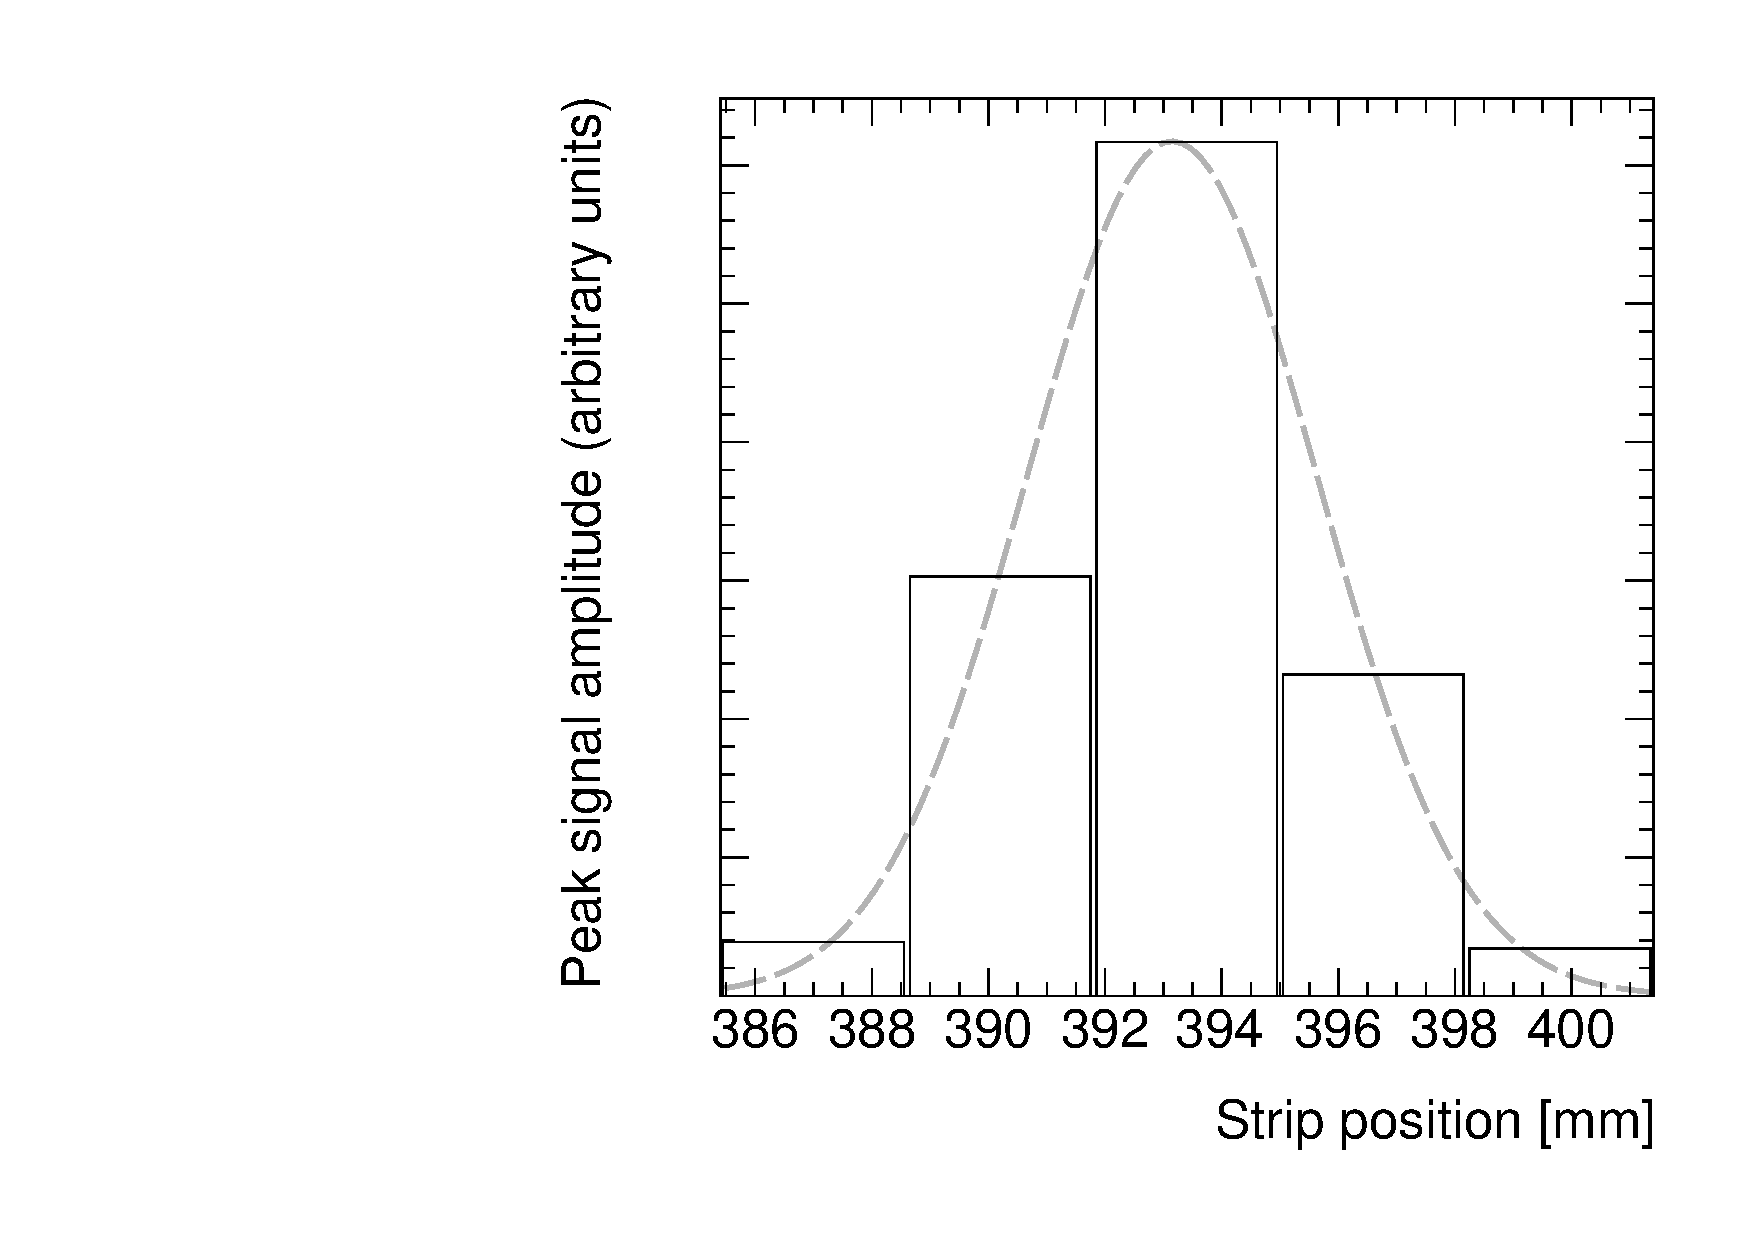
\includegraphics[width = 0.5\textwidth]{figures/sample_cluster_QL2C04_event5_layer2.pdf}
    \caption{A sample cluster resulting from the current picked up on a group of strips  after the passing of a muon (presumably). The grey curve is a Gaussian fit.}
    \label{fig:sample_cluster}
\end{figure}

Events are cut from the analysis if there are two clusters on one layer's set of strips (indicative of noise). Clusters are cut if the cluster size is lesser than three (which should not happen for real events thanks to neighbour triggering), and if the cluster size is greater than 25. After all the cuts on hits and clusters, roughly half as many muon tracks as triggers collected remain.

The uncertainty in the $y$-coordinate could have been taken as the fitted cluster mean's statistical uncertainty; however, after comparing the difference in cluster means for different fitting algorithms in appendix~\ref{sec:appendix_clustering_cluster_fit}, \SI{60}{\micro\meter} of uncertainty was assigned.

The coordinates of the avalanches' on all layers were used to reconstruct tracks in x and y respectively. The tracks were then used to calculate characterization metrics like electrode efficiency and spatial resolution, the details of which are discussed in~\cite{lefebvre_thesis}.

%TODO : Include hit and track map? - yes if Brigitte says you need a num_entries plot in chapter 3. You didn't include it because you never mention wire supports in TH2 analysis. But if you want to add num entries for clarity, include cluster map here. Cluster map > raw hits because less cuts and gets across the idea that x is just hit or no hit while y comes from clustering.  

% Edit count: Lia - 2, Brigitte - 0

% --------------------------------------------------
\section{Measuring relative local offsets}
% --------------------------------------------------

The offset of a strip from its nominal position can be modeled as a passive transformation. For each area of a strip layer, the local offset is the shift of the strip pattern in that area with respect to the nominal geometry.  Local offsets systematically change the set of strips nearest to muons passing through the area. The data preparation software assumes that strips are in their nominal positions, so the recorded muon $y$-position on layer $i$, $y_i$, is shifted opposite to the layer's local offset, $d_{local, i}$, by
% Maybe useful sentence?: The local offset is a result of the non-conformities in the strip pattern etching and inter-layer misalignments.
\begin{equation}
    y_i = y_{nom, i} - d_{local, i},
    \label{eqn:local_translation}
\end{equation}
% Maybe useful sentence?: The true position of individual cosmic muons is not known, and in the analysis the four detector planes float with respect to a software-implemented origin that is not associated with a fixed physical location.
where $y_{nom, i}$ is the position of the muon that would have been recorded on layer $i$ if there was no local offset. Equation~\ref{eqn:local_translation} ignores other factors that affect the cluster position, like position resolution. With cosmics data, the local offset is unknown and there was no external reference to measure $y_{nom, i}$. Therefore, only relative local offsets could be calculated. 

% Potential BREAK for Motivation section at beginning ^

The minimal relative coordinate system uses two reference or fixed layers~\cite{lefebvre_thesis}. The hits on the two fixed layers were used to create tracks that can be interpolated or extrapolated (polated) to the other two layers. The set of two fixed layers and the layer polated to are referred to as a tracking combination. The residual of track $i$, $\Delta_i$ is defined as,
\begin{equation}
    \Delta_i = y_{i} - y_{track, i},
    \label{eqn:residual}
\end{equation}

where $y_{track, i}$ is the polated track position. Track residuals are affected by the relative local offset in the area of each layer's hit. As an example, in figure~\ref{fig:fake_event_display}, the residual on layer 2 perhaps indicates that layer 2 is offset with respect to layers 1 and 4 in the area of the track. Of course, a single track residual says nothing of the real relative local offset because of the limited spatial resolution of the detectors and fake tracks caused by noise or delta rays. However, the mean of residuals for all tracks in a region will be shifted systematically by the local offsets between layers~\cite{lefebvre_thesis}. For a quadruplet with nominal geometry, the mean of residuals should be zero in all regions and for all reference frames, unlike the example regions in figure~\ref{fig:res_dist}. The value of the mean of residuals is a measure of the relative local offset of the layer with respect to the two fixed layers. The sign convention is such that the mean of residuals is opposite to the relative local offset.

\begin{figure}
    \centering
    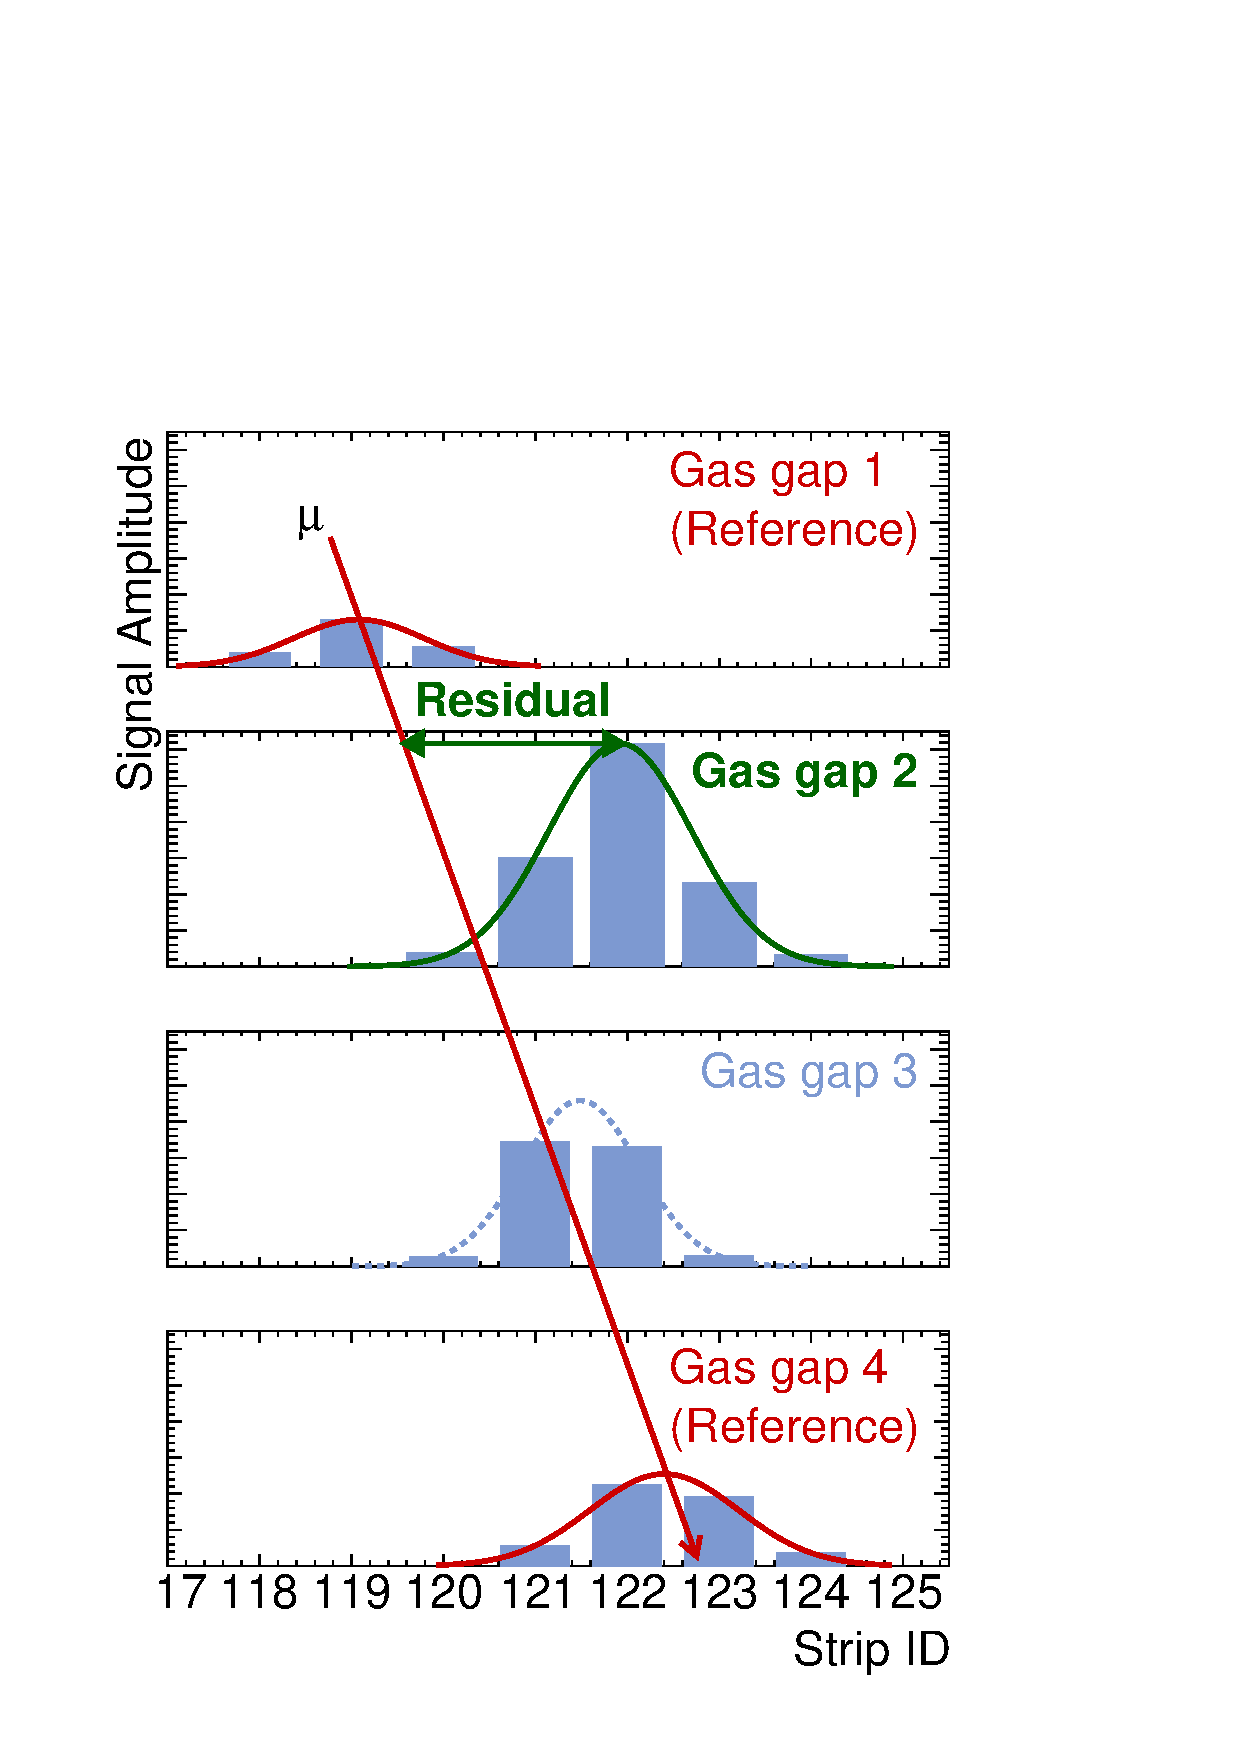
\includegraphics[width = 0.9\textwidth]{figures/figure_fake_event_display.pdf}
    \caption{Representation of a muon event recorded by an sTGC. The clusters are fit with a Gaussian and the mean is taken as the hit position. A track is built from the chosen reference layers, 1 and 4, and the residual calculated on layer 2. The clusters come from a real muon, but their positions were modified to highlight the residual on layer 2.}
    \label{fig:fake_event_display}
\end{figure}

\begin{figure}
\centering
\begin{subfigure}{.5\textwidth}
  \centering
  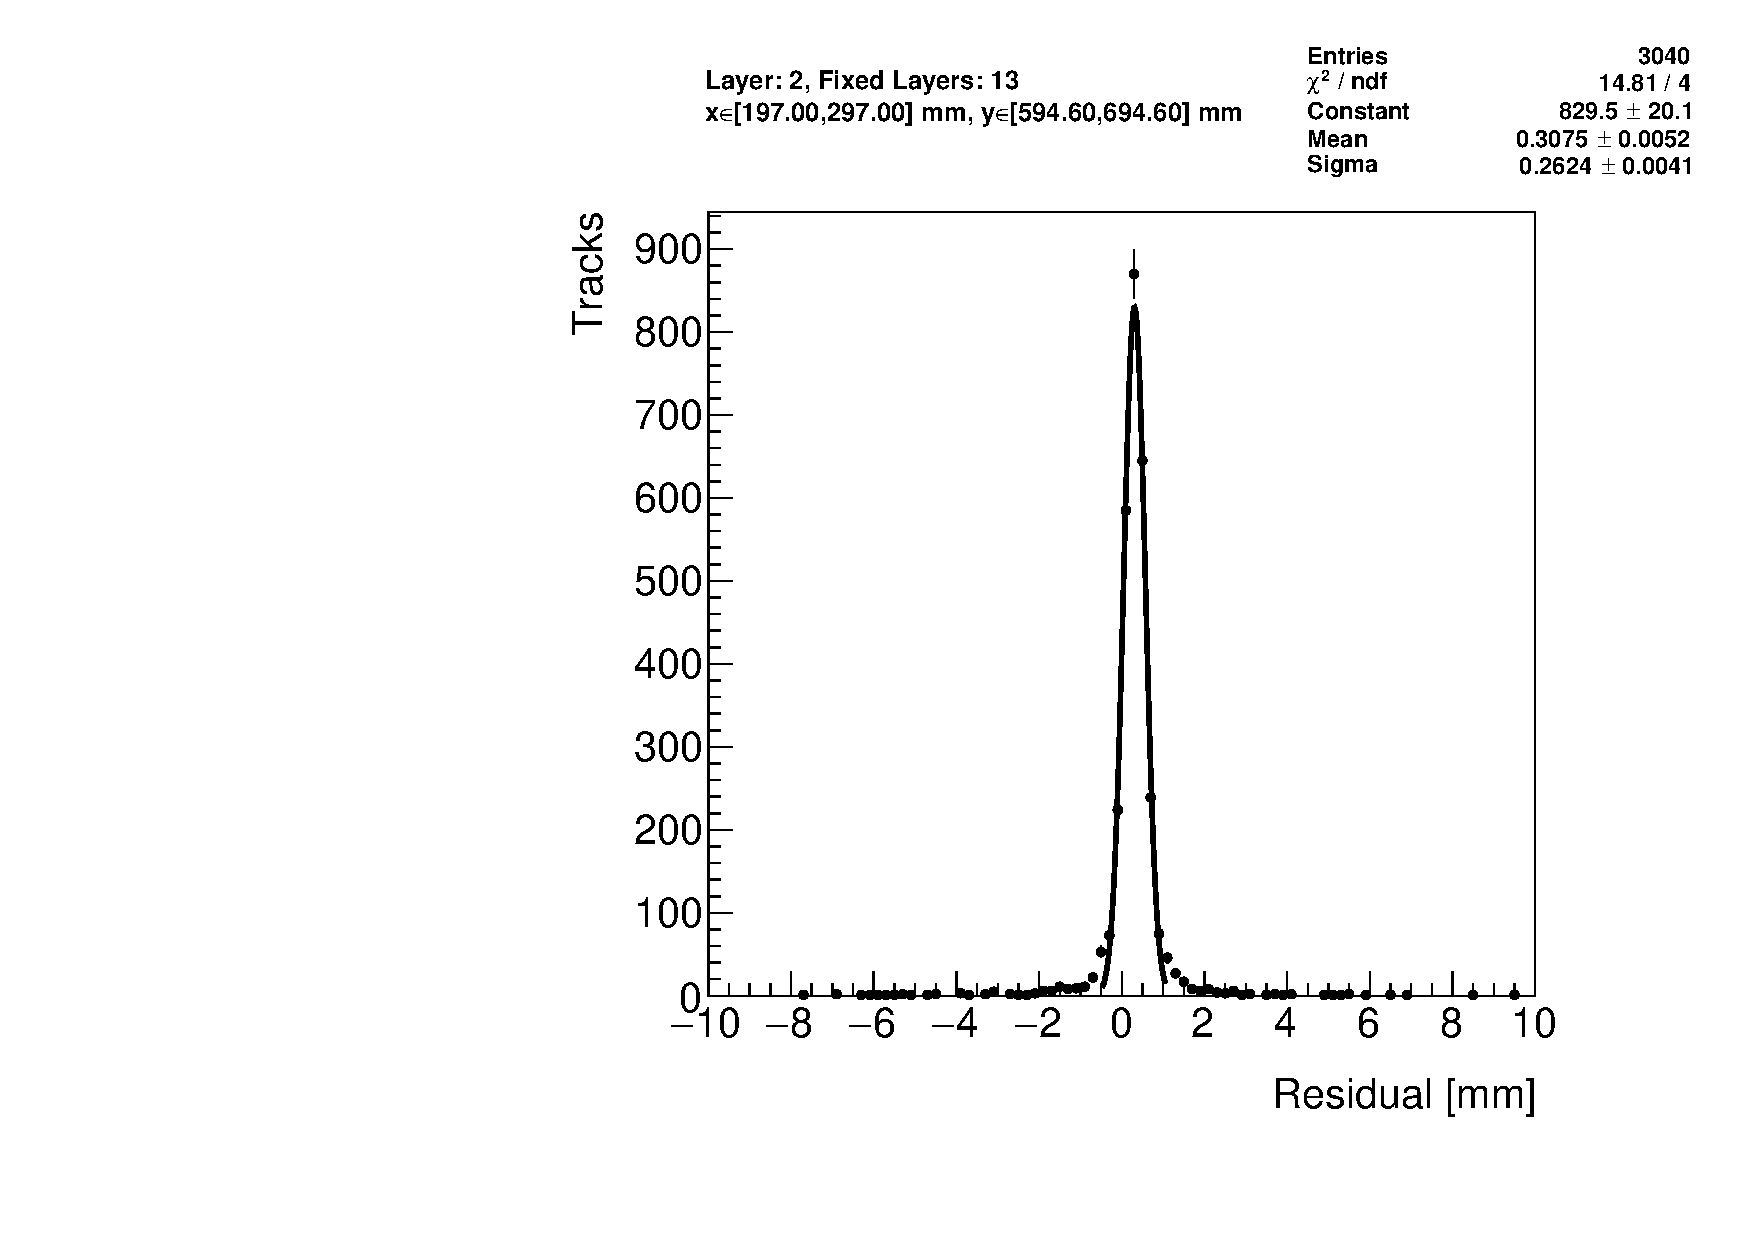
\includegraphics[width=\linewidth]{figures/figure_res_dist_QL2P11_3100V_2021-08-05_xbin_12_ybin_7_layer2_fixedlayers13.pdf}
  \caption{Tracks on layer 2, reference layers 1 and 3.}
  \label{fig:res_dist_L2_F13}
\end{subfigure}
\begin{subfigure}{.5\textwidth}
  \centering
  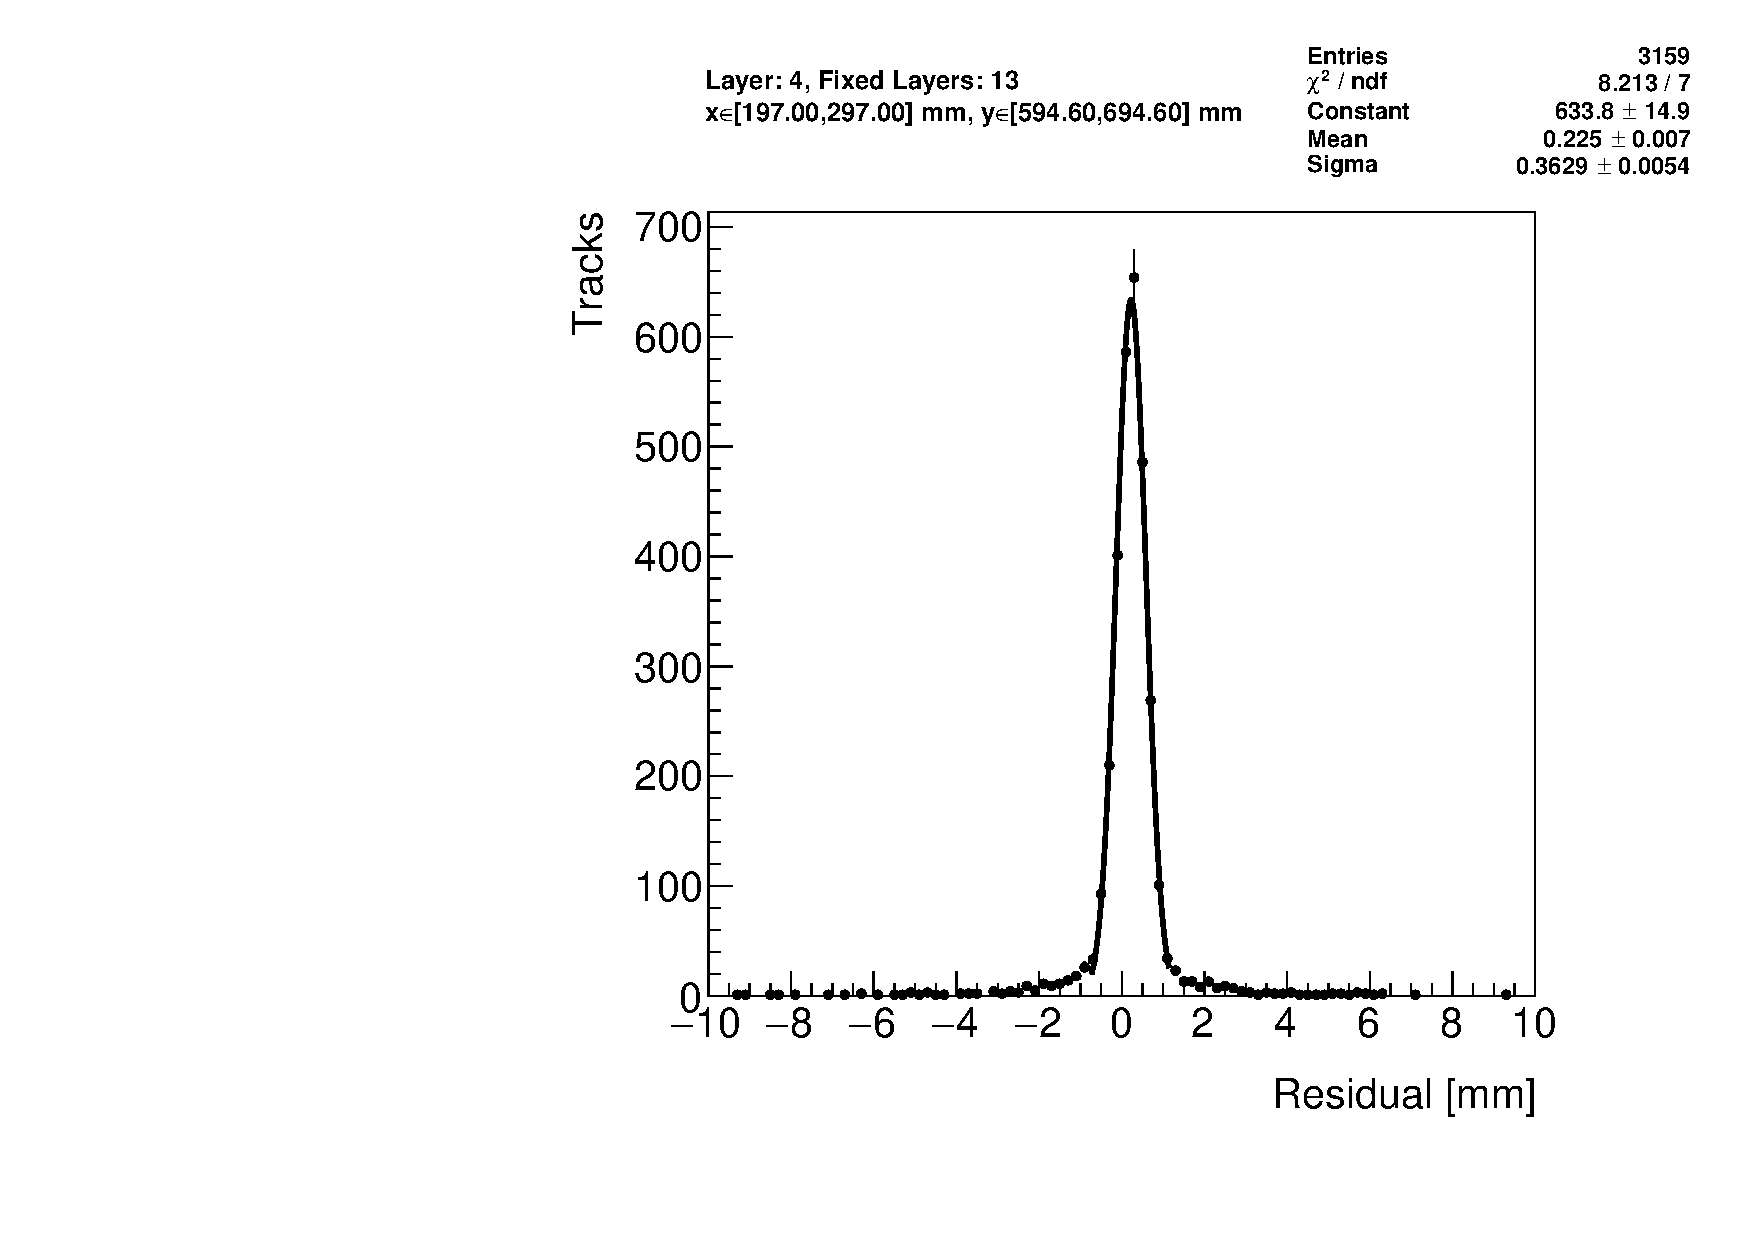
\includegraphics[width=\linewidth]{figures/figure_res_dist_QL2P11_3100V_2021-08-05_xbin_12_ybin_7_layer4_fixedlayers13.pdf}
  \caption{Tracks on layer 4, reference layers 1 and 3.}
  \label{fig:res_dist_L4_F13}
\end{subfigure}
\caption{Residual distribution in the region $x\in\left[197, 297\right],  y\in\left[594.6, 694.6\right]$~mm (\SI{100}{mm} by \SI{100}{mm} area) for two different tracking combinations. Data from quadruplet QL2.P.11.}
\label{fig:res_dist}
\end{figure}

To study the relative local offsets, residual distributions across each strip layer of a quadruplet for all tracking combinations were assembled and fitted. The residual distributions were wider for tracking combinations where the extrapolation lever arm was largest, as in the example distributions shown in figure~\ref{fig:res_dist}. In general, residual means from distributions of residuals with geometrically less favourable tracking combinations have larger statistical and systematic uncertainties. The bin size of \SI{200}{\micro\meter} for the distributions shown in figure~\ref{fig:res_dist} was chosen based on the uncertainty on residuals calculated from tracks on layer 4 (1) built from hits on layers 1 and 2 (3 and 4) given a cluster $y$-position uncertainty of \SI{60}{\micro\meter} (appendix~\ref{sec:appendix_clustering_track_residuals}), since these tracks yield residuals with the largest uncertainties.

A gaussian fit was used to extract the mean of the residual distributions. Theoretically, a double gaussian distribution is more apt, but for this analysis the gaussian fit was sufficient, as discussed in appendix~\ref{appendix:systematics_res_fit_fcn}.

The area of the region of interest was \SI{100}{\milli\meter} by \SI{100}{\milli\meter}. The size balanced the amount of tracks falling in the region of interest to give a small statistical uncertainty on the extracted mean while being smaller than the order on which local offsets were expected to change significantly. The change in local offsets over the surface of a layer can be modeled using global alignment parameters. Using a base alignment model with a global offset and rotation of each strip layer, ``significantly'' was defined by the distance in $x$ that a large but possible rotation of \SI{1000}{\micro\radian} would change the local offset by more than \SI{50}{\micro\meter}~-- half the required position resolution of the sTGCs~\cite{nsw_tdr}.

% Original position of this paragraph
% It is only possible to calculate relative local offsets with cosmics data because there was no external reference to measure positions on all layers with respect to. As an example, assuming that the residual on layer 2 in figure~\ref{fig:fake_event_display} is representative of the relative local offset, the residual on layer 2 could be caused by the strips on layer 2 being misaligned from nominal, but it could also be caused by strips on layers 1 and 4 being misaligned from nominal while the strips on layer 2 are in their nominal positions! Any number of combinations of local offsets on layers 1, 2 and 4 could produce the residual on layer 2. The value of relative local offset measurements will be shown and discussed throughout this work.

% --------------------------------------------------
\section{Visualizing relative alignment between layers}
% --------------------------------------------------

The mean of residuals was plotted across entire strip layers for every tracking combination to get a picture of the how relative local offsets change over the layers' surface. Figure~\ref{fig:res_mean_th2} shows the mean of residuals on layer 2 with reference layers 1 and 3 for two different quadruplets, referred to as QL2.P.11 and QL2.P.8, for \SI{100}{mm} by \SI{100}{mm} areas across the surface of layer 2. To understand these plots, realize that the Gaussian mean of the distribution in figure~\ref{fig:res_dist_L2_F13} is the entry in area bin $x\in\left[197, 297\right],  y\in\left[594.6, 694.6\right]$~mm in figure~\ref{fig:res_mean_th2_ql2p11}.

\newpage
\thispagestyle{empty}
\newgeometry{top=0.5in,bottom=0.5in}
\begin{figure}
\centering
\begin{subfigure}{\textwidth}
  \centering
  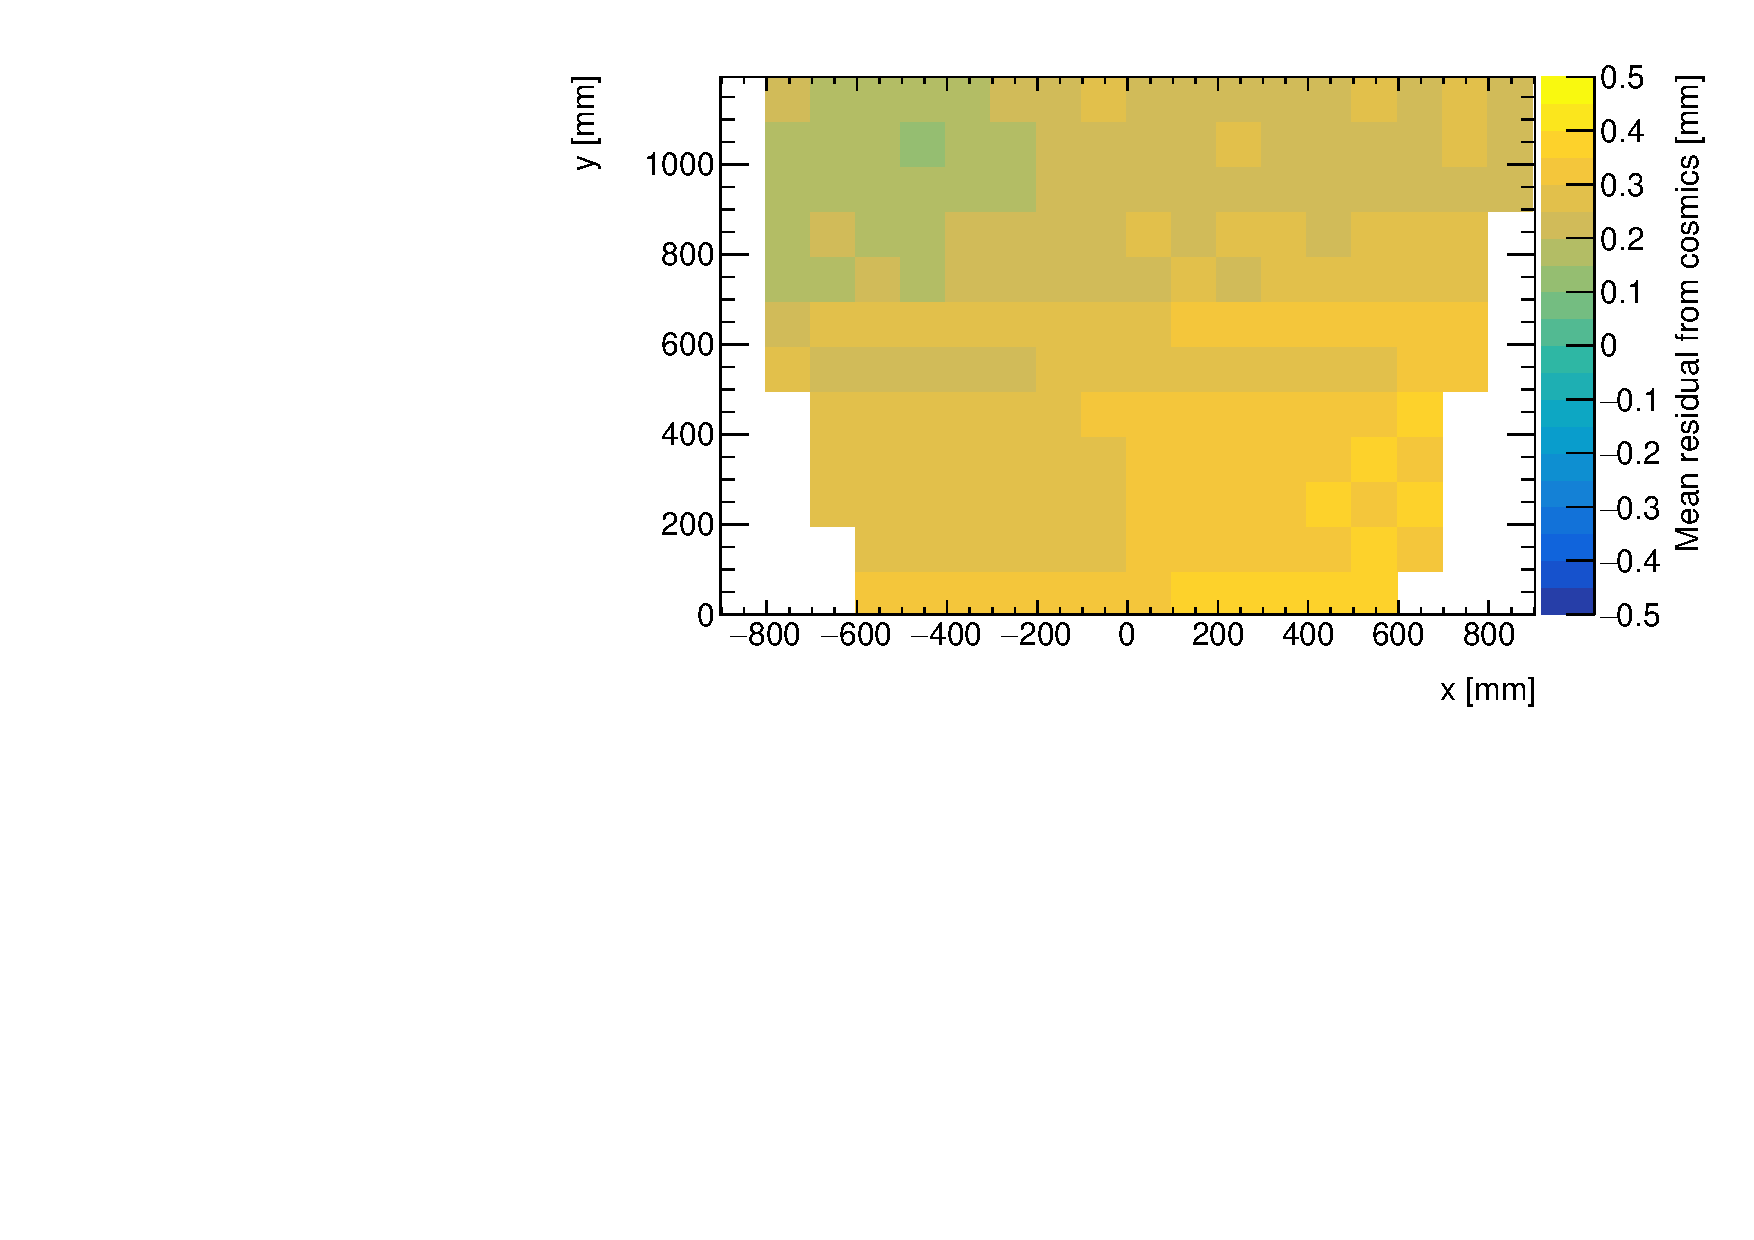
\includegraphics[width=\linewidth]{figures/figure_QL2P11_3100V_2021-08-05_th2_means_layer2_fixedlayers13.pdf}
  \caption{Mean of residuals of tracks on layer 2, reference layers 1 and 3, for QL2.P.11.}
  \label{fig:res_mean_th2_ql2p11}
\end{subfigure}%
\vspace*{\floatsep}
\begin{subfigure}{\textwidth}
  \centering
  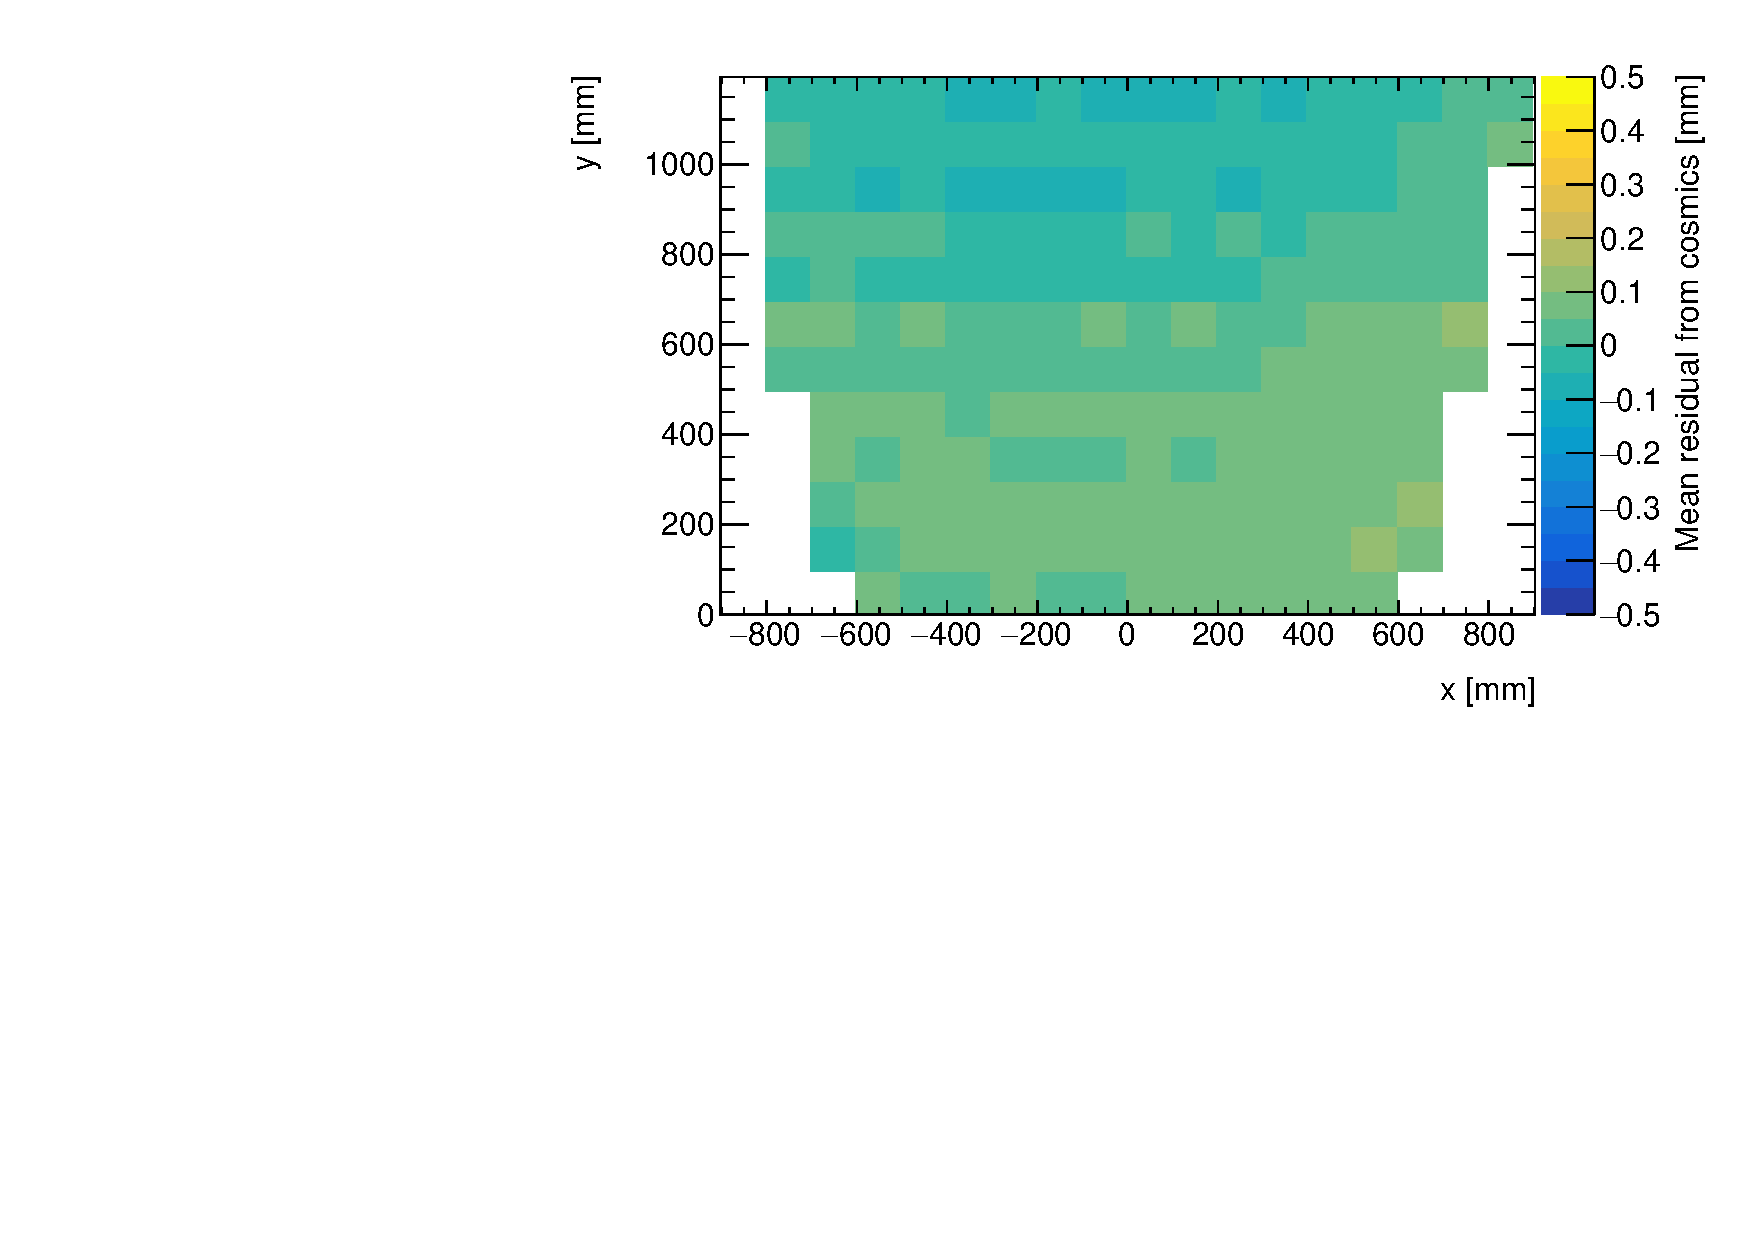
\includegraphics[width=\linewidth]{figures/figure_QL2P08_3100V_2021-08-03_th2_means_layer2_fixedlayers13.pdf}
  \caption{Mean of residuals of tracks on layer 2, reference layers 1 and 3, for QL2.P.8.}
  \label{fig:res_mean_th2_ql2p8}
\end{subfigure}
\caption{Mean of residuals in each \SI{100}{\milli\meter} by \SI{100}{\milli\meter} bin over the area of the layer 2 cathode board. The entry in $x\in\left[197, 297\right],  y\in\left[594.6, 694.6\right]$~mm of figure~\ref{fig:res_mean_th2_ql2p11} corresponds to the fitted Gaussian means in figures~\ref{fig:res_dist_L2_F13}. The mean of residuals in each area is inversely proportional to the relative local offset of layer 2 with respect to layers 1 and 3.}
\label{fig:res_mean_th2}
\end{figure}
\newpage
\restoregeometry

Many of the residual means are non-zero and change smoothly over the layer, indicating that there are relative local offsets stemming from misalignments between entire strip layers. Given that the residual mean changes with $x$ in figure~\ref{fig:res_mean_th2_ql2p11}, there is likely a rotation of layer 2 with respect to layers 1 and 3 on QL2.P.11, combined with an offset of the entire layer. The residual means are smaller in figure~\ref{fig:res_mean_th2_ql2p8} indicating that QL2.P.8 is less misaligned overall than QL2.P.11; however the relative local offsets range between $\pm$\SI{200}{\micro\meter} so they are still significant considering the order on which the chambers must be sensitive to position, $\sim$\SI{100}{\micro\meter}.

% --------------------------------------------------
\section{Systematic uncertainty}
% --------------------------------------------------
\label{sec:cosmics_sys_uncerts}

The statistical uncertainty on the local residual means was typically around \SI{10}{} - \SI{20}{\micro\meter}, and appendix~\ref{appendix:statistics} shows that the analysis was not statistically limited by the number of triggers collected for each quadruplet. The systematic uncertainties were more significant. 

Systematic uncertainties were assigned per tracking combination as the RMS of the distribution of the difference in residual means each calculated in a different way. For example, the RMS associated with fitting the local residual distributions with a Gaussian or double Gaussian is \SI{25}{\micro\meter} for the geometrically least favourable tracking combinations. The distribution is shown in appendix~\ref{appendix:systematics_res_fit_fcn}. For geometrically similar tracking combinations (like: tracks on layer 1 built from hits on layers 3 and 4, and tracks on layer 4 built from hits on layers 1 and 2), the systematic uncertainty was assigned as the average RMS of both.

Other choices were: whether to use data collected at 2.9~kV or 3.1~kV (both are collected at McGill); what cluster fitting algorithm to use; and whether or not to apply a differential non-linearity (DNL) correction to the cluster $y$-positions~\cite{abusleme_performance_2016}. A systematic uncertainty was assigned using the method above to account for the effect of each choice and quantify the robustness of the mean of residuals. The reasons for each choice are listed below.

Data taken at 3.1~kV was used over 2.9~kV because the strip and wire tracking efficiency increases with higher voltage~\cite{lefebvre_thesis} (appendix~\ref{appendix:systematics_2900V_vs_3100V}).

The \package{Minuit2} package~\cite{hatlo_developments_2005} was used to fit clusters over Guo's method~\cite{guo_simple_2011} because it provided automatic statistical uncertainty estimates and is the standard fit algorithm of \package{ROOT}~\cite{ROOT_paper} (appendix~\ref{appendix:systematics_cluster_fit_fcn}).

The DNL correction was not applied because its effect on the residual means was negligible (appendix~\ref{appendix:systematics_dnl}).

A summary of the systematic uncertainties assigned to the mean of residuals for each tracking combination is given in table~\ref{tab:sys_uncerts}.

\begin{table}

\begin{tabularx}{\textwidth} {
 | >{\raggedright\arraybackslash}X
 | >{\raggedright\arraybackslash}X 
 | >{\raggedright\arraybackslash}X 
 | >{\raggedright\arraybackslash}X 
 | >{\raggedright\arraybackslash}X 
 | >{\raggedright\arraybackslash}X 
 | >{\raggedright\arraybackslash}X | }
 
 \hline
 \textbf{Tracking geometry} & \textbf{Residual distribution fit function (\ref{appendix:systematics_res_fit_fcn})} & \textbf{Cosmics data collection voltage (\ref{appendix:systematics_2900V_vs_3100V})} & \textbf{Cluster fit algorithm (\ref{appendix:systematics_cluster_fit_fcn})} & \textbf{Apply DNL correction or not (\ref{appendix:systematics_dnl})} & \textbf{Total} \\ 
 \hline
 \hline 
   Similar to layer 3, fixed layers 1, 2 & 0.01 & 0.04 & 0.02 & 0.01 & \textbf{0.05} \\
 \hline
   Similar to layer 4, fixed layers 1, 2 & 0.03 & 0.01 & 0.03 & 0.01 & \textbf{0.10} \\
 \hline
    Similar to layer 2, fixed layers 1, 3 & 0.01 & 0.02 & 0.01 & 0.000 & \textbf{0.03} \\
 \hline
    Similar to layer 4, fixed layers 1, 3 & 0.01 & 0.04 & 0.01 & 0.01 & \textbf{0.04} \\
 \hline
    Similar to layer 2, fixed layers 1, 4 & 0.01 & 0.04 & 0.01 & 0.01 & \textbf{0.04} \\
 \hline
 
\end{tabularx}
\caption{Systematic uncertainty assigned for each analysis option, detailed in appendix~\ref{appendix:systematics}.}
\label{tab:sys_uncerts}
\end{table}

The uncertainty in each mean of residuals was assigned as the sum in quadrature of the statistical uncertainty in the mean and the appropriate systematic uncertainty for the tracking combination. 

% --------------------------------------------------
\section{Discussion}
% --------------------------------------------------

Cosmics data is being used to calculate relative alignment parameters using two other methods~\cite{lefebvre_thesis}. The results of this analysis could be cross-checked with the other methods; however the studies in appendix~\ref{appendix:systematics} show that the residual means are robust, so the comparison was not prioritized.

Given that the uncertainty in the residual means is lesser than or near to the order of the required position resolution of the sTGCs (\SI{100}{\micro\meter}~\cite{nsw_tdr}) they are relevant input for alignment studies.

The relative local offsets as calculated from the mean of residual distributions provide a complete picture of the relative alignment between detectors planes. In fact, cosmic muon testing is the only characterization technique where the entire surface of quadruplet layers can be probed since muons hits are distributed almost uniformly; the CMM~\cite{carlson_results_2019} and x-ray methods~\cite{lefebvre_precision_2020} depend on measurements at reference points, and test beams only have a limited beam spot~\cite{abusleme_performance_2016}. By looking at 2D-histograms of residual means like figure~\ref{fig:res_mean_th2} for all tracking combinations, it is easy to identify quadruplets that suffer large relative misalignment since many residual means differ significantly from zero. Moreover, the pattern in the residual means can be used to motivate a physical interpretation of misalignments. The residual means can be used as a reference, cross check, or input in other alignment studies.

Relative local offsets cannot be used to position strips in the absolute ATLAS coordinate system because there was no external reference to measure positions on all layers with respect to. The lack of external reference means that there is not enough information to unfold relative local offsets into absolute local offsets (with respect to the nominal quadruplet geometry). As an example, assuming that the residual on layer 2 in figure~\ref{fig:fake_event_display} is representative of the absolute value of the relative local offset, the residual on layer 2 could be caused by the strips on layer 2 being misaligned from nominal, but it could also be caused by strips on layers 1 and 4 being offset from nominal while the strips on layer 2 are in their nominal positions! Any number of combinations of local offsets on layers 1, 2 and 4 could produce the residual on layer 2. Absolute local offsets must be calculated another way.